% This file was created with tikzplotlib v0.10.1.
\definecolor{mycolor1}{rgb}{0.00000,0.44700,0.74100}%
\definecolor{mycolor2}{rgb}{0.85000,0.32500,0.09800}%
\definecolor{mycolor3}{rgb}{0.92900,0.69400,0.12500}%
\definecolor{mycolor4}{rgb}{0.49400,0.18400,0.55600}%
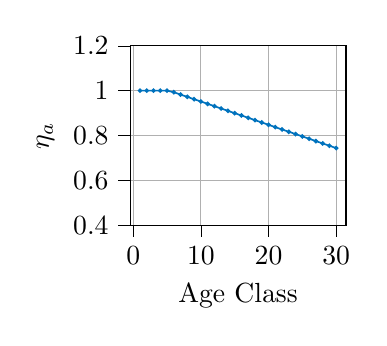
\begin{tikzpicture}

\definecolor{darkgray176}{RGB}{176,176,176}
\definecolor{steelblue31119180}{RGB}{31,119,180}

\begin{axis}[
/pgf/number format/1000 sep={},
scale = 0.4,
tick align=outside,
tick pos=left,
x grid style={darkgray176},
xlabel={Age Class},
xmajorgrids,
xmin=-0.45, xmax=31.45,
xtick style={color=black},
y grid style={darkgray176},
ylabel={$\eta_a$},
ymajorgrids,
ymin=0.4, ymax=1.2,
ytick style={color=black}
]
\addplot [semithick, mycolor1, mark=*, mark size=.5, mark options={solid}]
table {%
1 1
2 1
3 1
4 1
5 1
6 0.99298212
7 0.98260041
8 0.9722187
9 0.96183699
10 0.95145528
11 0.94107357
12 0.93069186
13 0.92031015
14 0.90992844
15 0.89954673
16 0.88916502
17 0.87878331
18 0.8684016
19 0.85801989
20 0.84763818
21 0.83725647
22 0.82687476
23 0.81649305
24 0.80611134
25 0.79572963
26 0.78534792
27 0.77496621
28 0.7645845
29 0.75420279
30 0.74382108
};
\end{axis}

\end{tikzpicture}
